% \newpage
\section{Evaluation} \label{sec:eval}

\begin{figure}[t]
\centering
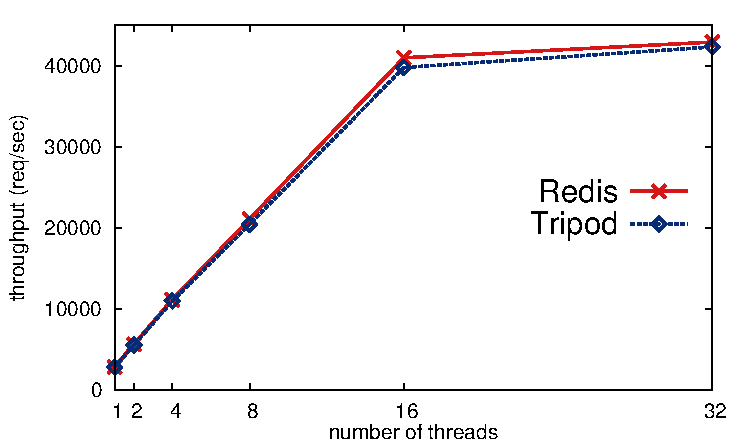
\includegraphics[width=0.9\textwidth]{figures/throughput}
\vspace{-.10in}
\caption{\small {\em \xxx throughput compared to the unreplicated 
execution.}}
\vspace{-.20in}
\label{fig:tput}
\end{figure}
 
\begin{figure}[t]
\centering
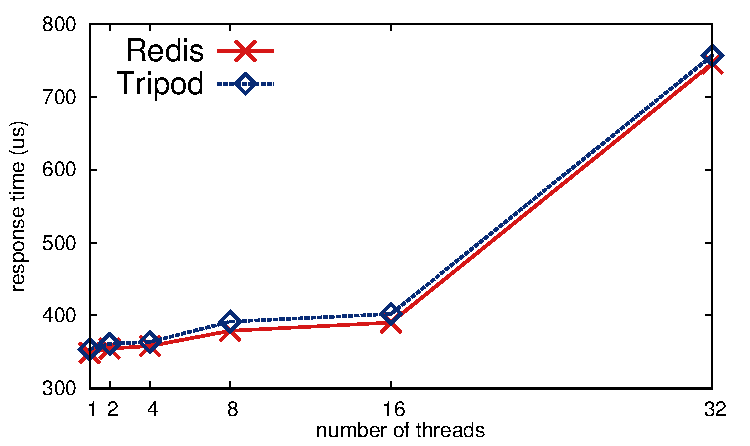
\includegraphics[width=0.9\textwidth]{figures/latency}
\vspace{-.10in}
\caption{\small {\em \xxx response time compared to the unreplicated 
execution.}}
\vspace{-.20in}
\label{fig:latency}
\end{figure}

As part of \xxx's development, we have implemented a fast RDMA-enabled \paxos 
protocol~\cite{falcon:github} for general applications. We evaluated this 
protocol with \redis~\cite{redis}, a popular key-value store. We chose \redis 
because it complies with a social-networking platform setting. For instance, 
Twitter uses \mesos as its scheduler and runs \redis as its core key-value 
store. Key-value stores are also widely used 
in critical, financial applications~\cite{nosql:finance,nosql:racs14}.

% Evaluation machine and workloads.
Our evaluation used three Dell R430 servers as SMR replicas. Each server has 
Linux 3.16.0, 2.6 GHz Intel Xeon CPU with 24 hyper-threading cores, 64GB 
memory, and 1TB SSD. Each machine has a Mellanox ConnectX-3 Pro Dual Port 40 
Gbps NIC. These NICs are connected using the Infiniband RDMA architecture.

To mitigate network latency of public network, benchmarks were ran 
in a Dell R320 server (the application scheduler machine), with Linux 3.16.0, 
2.2GHz Intel Xeon 12 hyper-threading cores, 32GB memory, and 160GB SSD. This 
server connects with the server machines with 1Gbps bandwidth LAN. The average 
\v{ping} latency between the client machine and a server machine is 301 \us. A 
larger network latency (\eg, sending job requests from WAN) will further 
mask \xxx's overhead.

To perform a stress testing on \xxx's input consensus protocol, we chose 
\redis's own benchmark to spawn a workload with 50\% SET and 50\% GET 
operations. We chose such a significant portions of writes because SET 
operation contains more bytes than a GET.

In our evaluation, we did not need to modify \redis's code and it ran with 
\xxx's replication protocol. Figure~\ref{fig:tput} shows \xxx's throughput and 
Figure~\ref{fig:latency} response time. We varied the number of concurrent 
client connections for each server program by from one to 32 threads. Overall, 
compared to \redis's unreplicated executions, \xxx merely incurred a mean 
throughput overhead of \tputoverhead. 

To deeply understand \xxx's performance overhead, we collected the number of 
socket call events and consensus durations on the leader controller side. Given 
10K requests and 8 concurrent connections, \redis spawned 10,016 socket calls, 
each of which invoked a \paxos consensus. The average received data bytes in 
these socket calls were 42.0 (\eg, inputs from \recv). The average consensus 
latency for these calls were 9.9 \us because consensus were done by RDMA WRITEs 
across the leader and standby masters. These initial results suggest that \xxx 
has the potential to provide a fast \paxos replication service to general 
applications with low overhead. 

% Results: tput, latency.

% \subsection{Performance Overhead of \xxx's \paxos protocol} \label{sec:overhead}



% \subsection{Response Times in Critical Application Workloads} 
% \label{sec:workload}
% 
% TBD.

